\documentclass[12pt]{article}
\usepackage{graphicx} 
\usepackage{float}

\title{CodeStories} 

\author{Roelof Sol, Salim Salmi, Maarten van Beek}

% Include the date command, but leave its argument blank.

\date{}
\begin{document} 
\maketitle
\section{Abstract}
\section{Introduction}
The current process of understanding software projects can be a cumbersome practice. 

We strive to make documentation more interactive and enjoyable through interactive storytelling. A practice in which the user 
decides with which information he or she is provided and makes it possible for the user to gradually guide him- or herself 
through the project.  

\section{Research}
\subsection{Project Description}
Formal description of the project. 

\subsection{Existing solutions}
Describe the existing solutions to interactive documentation.

\subsection{User Stories}
User stories to illustrate the use of the application. 

\subsection{Requirements}
Our requirements in MoSCoW

\subsection{Choice of technologies}
Angular, Karma, JS-Interpreter, Ace Editor

\subsection{Conclusions}

\section{Project Planning}
\subsection{Scrum}
\subsection{Testing}
\subsection{Time Planning}

\section{Product Design}
\subsection{Introduced Concepts}
CAST, VCode
\subsection{UML Diagram}
We use the Model View Controller structure that is natural to Angular for our application. 
\begin{figure}[H]
 \centering
 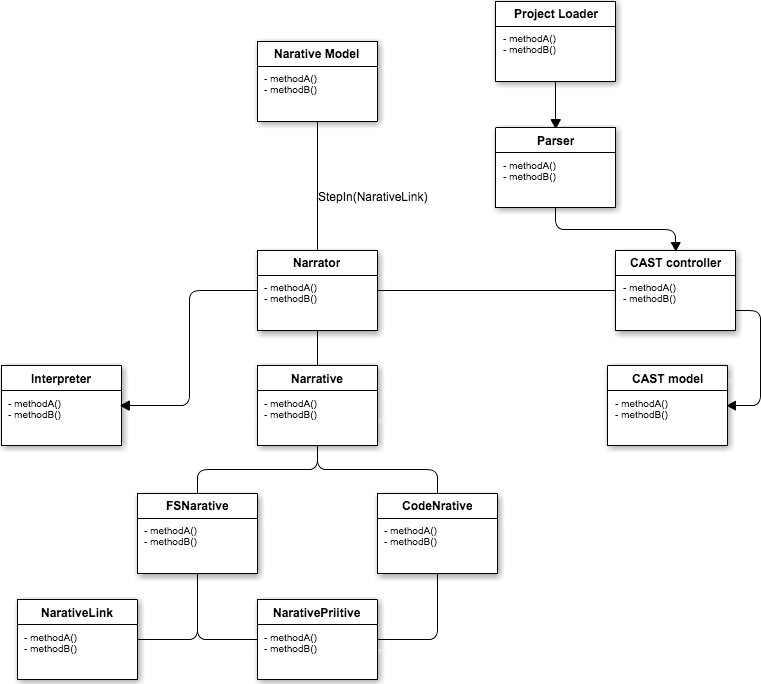
\includegraphics[width=0.8\textwidth]{uml-webos.png}
 \caption{CodeStories UML Diagram}
 \label{fig:uml_diagram}
\end{figure}

\section{Conclusion}

\section{Recommendations}

\section{Glossary}
\end{document}
